\section{divagazione sui frattali autosimili}

In questo capitolo mostriamo una applicazione geometrica del teorema delle contrazioni.
Considereremo uno spazio metrico i cui punti sono le figure geometriche
e vedremo che i frattali autosimili non sono altro che punti fissi
di opportune mappe contrattive.

\begin{definition}
Siano $A$ e $B$ sottoinsiemi non vuoti di $\RR^n$.
Definiamo la \emph{distanza di Hausdorff}
\mymargin{distanza di Hausdorff}
\index{distanza!di Hausdorff}
tra $A$ e $B$ come:
\[
  d_{\H}(A,B) = \max\ENCLOSE{\sup_{a\in A}\inf_{b\in B} \abs{a-b}, \sup_{b\in B} \inf_{a\in A} \abs{a-b}}.
\]

Definiamo
\[
 \K(\RR^n) = \ENCLOSE{A \subset \RR^n \colon \text{$A$ chiuso, limitato, non vuoto}}.
\]
\end{definition}

\begin{theorem}[caratterizzazione della distanza di Hausdorff]
Se $A$ e $B$ sono compatti di $\RR^n$ (cioè chiusi e limitati) allora
per ogni $r \in \RR$
si ha
\[
  d_\H(A,B) \le r
\]
se e solo se valgono entrambe le seguenti proprietà:
\begin{enumerate}
\item per ogni $a\in A$ esiste $b\in B$ tale che $\abs{a-b}\le r$;
\item per ogni $b\in B$ esiste $a\in A$ tale che $\abs{a-b}\le r$.
\end{enumerate}
\end{theorem}
%
\begin{proof}
Per ogni compatto non vuoto $A$ e per ogni $x\in \RR^n$ definiamo
la distanza tra il punto $x$ e l'insieme $A$ come:
\[
  d(x,A) = \min_{a\in A} \abs{x-a}.
\]
Il minimo esiste in quanto $A$ è compatto e $a\mapsto d(x,a)$ è una funzione continua. Fissato $A$ la funzione $x\mapsto d(x,A)$ è anch'essa continua, anzi è $1$-lipschitziana. Infatti se $x'\in \RR^n$ esiste $a'\in A$ tale che $d(x',A) = d(x',a')$ e dunque
\[
  d(x,A) = \min_{x\in A} \abs{x-a} \le \abs{x-a'} \le \abs{x-x'} + \abs{x'- a'}
   = \abs{x-x'} + d(x',A)
\]
da cui $d(x,A) - d(x',A)\le \abs{x-x'}$.
Scambiando $x$ e $x'$ si ottiene anche la disuguaglianza inversa da cui la $1$-lipschitzianità di $d(x,A)$. Dunque sui compatti la funzione $d(x,A)$ assume sempre massimo e si ha:
\[
d_\H(A,B) = \max\ENCLOSE{\max_{a_\in A} d(a,B), \max_{b\in B} d(b,A)}.
\]

In particolare se $d_\H(A,B) \le r$ per ogni $a\in A$ si deve avere $d(a,B) \le r$ e per ogni $b\in B$ si deve avere $d(b,A) \le r$. Ma allora valgono le due proprietà dell'enunciato.

Viceversa se vale la proprietà 1.\ allora $d(a,B)\le r$ e se vale la 2.\ $d(b,A)\le r$ e di conseguenza $D_\H(A,B) \le r$.
\end{proof}

\begin{theorem}[distanza di Hausdorff]
La distanza di Hausdorff $d_\H$ è una distanza su $\K(\RR^n)$ e lo spazio metrico $\K(\RR^n)$ è completo.
\end{theorem}
%
\begin{proof}
Chiaramente se $A,B$ sono non vuoti si ha $d_\H(A,B) \ge 0$.
Inoltre, in base alla caratterizzazione del teorema precedente è facile osservare che $d_\H(A,B) < +\infty$.

Se $d_\H(A,B) = 0$ significa che per ogni $a\in A$ esiste $b\in B$ tale che $\abs{a-b}=0$. Cioè $b=a$. Dunque $A\subset B$. Scambiando i ruoli di $A$ e $B$ si ottiene anche $B\subset A$ da cui $A=B$.

Che sia $d_\H(A,B) = d_\H(B,A)$ è ovvio in quanto la definizione è simmetrica in $A$ e $B$.

Verifichiamo ora la disuguaglianza triangolare. Siano $A,B,C$ tre compatti non vuoti. Per ogni $a\in A$ esiste $b\in B$ tale che $\abs{a-b} \le d_\H(A,B)$ e per tale $b \in B$ esiste un $c\in C$ tale che $\abs{b-c} \le d_\H(B,C)$. Dunque per ogni $a\in A$ esiste un $c\in C$ tale che
\[
  \abs{a-c} \le \abs{a-b} + \abs{b-c} \le d_\H(A,B) + d_\H(B,C).
\]
Scambiando i ruoli di $A$ e $C$ si ottiene anche la condizione simmetrica e dunque, per la caratterizzazione della distanza di Hausdorff si ottiene la disuguaglianza triangolare:
\[
  d_\H(A,C) \le d_\H(A,B) + d_\H(B,C).
\]

Abbiamo quindi verificato che $d_\H$ è una distanza su $\K(\RR^n)$. Verifichiamo ora che $\K(\RR^n)$ è completo.

Sia $A_k\in\K(\RR^n)$ una successione di Cauchy.
Senza perdita di generalità possiamo supporre che
\[
  d_\H(A_k,A_{k+1}) \le \frac{1}{2^k}.
\]
Infatti essendo $A_k$ di Cauchy è possibile trovarne una sottosuccessione con tale proprietà, e se poi dimostriamo che la sottosuccessione converge allora l'intera successione, essendo di Cauchy, deve convergere.

Consideriamo come candidato limite l'insieme di tutti i possibili limiti di punti degli insiemi $A_k$:
\[
  A = \ENCLOSE{x\in \RR^n
  \colon \exists x_k \in A_k\colon x_k \to x}.
\]

Per prima cosa vogliamo verificare che $A$ non è vuoto. Scelto un punto qualunque $a_0 \in A_0$ esiste $a_1 \in A_1$ tale che $\abs{a_0 - a_1} = d_\H(A_0,A_1)$. Iterando otteniamo una successione di punti $a_k \in A_k$ tale che $\abs{a_k - a_{k+1}} \le d_\H(A_k,A_{k+1}) \le 1/2^k$.
Dunque $a_k$ è una successione di Cauchy in $\RR^n$ ed essendo $\RR^n$ completo dovrà convergere ad un punto $a$ che quindi è un punto di $A$.

Avendo assunto $d_\H(A_k, A_{k+1}) < 1/2^k$ si ottiene (sommando la serie geometrica):
\[
 d_\H(A_k, A_n) \le \sum_{j=k}^{n-1} d_\H(A_j, A_{j+1}) \le \frac{2}{2^k}\qquad \text{se $n>k$}.
\]
Questo ci permette di dimostrare che per ogni $a\in A$ e per ogni $k\in \NN$ esiste $a_k \in A_k$ tale che
$\abs{a - a_k}\le 4/2^k$. Infatti se a distanza $4/2^k$ non ci fossero punti di $A_k$ allora a distanza $2/2^k$ non ci potrebbero essere punti di $A_n$ per nessun $n>k$ in quanto visto che $d_\H(A_k,A_n) \le 2/2^k$ se ci fosse un punto di $A_n$ a distanza inferiore a $2/2^k$ ci dovrebbe anche essere un punto di $A_k$ a distanza inferiore a $4/2^k$. Ma questo è impossibile perché per come è definito $A$ deve esistere $x_n \in A_n$ tale che $x_n \to a$. Abbiamo quindi mostrato che
\[
  \sup_{a\in A} \inf_{b\in A_k} \abs{a-b} \le 4/2^k \to 0.
\]

Viceversa ci proponiamo di mostrare che per ogni $p \in A_k$ esiste $a \in A$ tale che $\abs{p-a} < 2/2^k$.
Visto che $d_\H(A_{j+1},A_j) \le 1/2^j$
possiamo infatti costruire a partire da $a_k=p \in A_k$
una successione $a_j \in A_j$ con $j > k$, tale che $d(a_{j+1},a_j) \le 1/2^j$. Tale successione è di Cauchy
quindi converge: $a_j \to a$
e il suo limite $a$ è quindi un punto di $A$ e si ha
\[
  \abs{a-p} \le \sum_{j=k}^\infty \abs{a_j - a_{j+1}}
    \le \sum_{j=k}^\infty \frac{1}{2^j} \le \frac{2}{2^k}.
\]
Abbiamo quindi dimostrato che
\[
  \sup_{b\in a_k} \inf_{a\in A} \abs{a-b} \le 2/2^k \to 0
\]
e quindi $d_\H(A_k,A)\to 0$.

Ci rimane solo da mostrare che $A$ è un insieme chiuso.
Presa una successione di punti $x_k\in A$ convergente $x_k\to x$, dobbiamo mostrare che $x\in A$. Per ogni $x_k\in A$ per quanto già detto sappiamo esistere $a_k \in A_k$ tale che $\abs{a_k-x_k}\le 4/2^k$. Ma allora $\abs{a_k-a} \le 4/2^k + \abs{x_k-a} \to 0$ e quindi $a_k\to a$ da cui $a\in A$.
 \end{proof}

\begin{theorem}[frattali autosimilari]
Siano $\phi_1, \dots, \phi_N \colon \RR^n \to \RR^n$ contrazioni (cioè funzioni lipschitziane con costante di lipschitz inferiore ad $1$).
Allora
esiste un unico insieme $C\subset \RR^n$ chiuso e limitato tale che
\[
  C = \bigcup_{k=1}^N \phi_k(C).
\]
\end{theorem}
%
\begin{proof}
Basterà dimostrare che la funzione $T\colon \K(\RR^n)\to \K(\RR^n)$ definita da
\[
  T(A) = \bigcup_{k=1}^N \phi_k(C)
\]
è una contrazione: dopodiché sapendo che $\K(\RR^n)$ è completo il risultato è conseguenza diretta del teorema di punto fisso di Banach-Caccioppoli.

Ogni $\phi_k$ per ipotesi è una contrazione, cioè
per ogni $a,b\in X$
\[
  \abs{\phi_k(a)-\phi_k(b)} \le L_k \abs{a-b}
\]
con $L_k< 1$. Posto $L=\max \ENCLOSE{L_1, \dots, L_N} < 1$ vogliamo dimostrare che $T$ è $L$-lipschitziana (e dunque una contrazione). Siano $A,B \in \K(\RR^n)$ e sia $d = d_\H(A,B)$. Preso $a' \in T(A)$ dovrà esistere $k$ tale che $a' \in \phi_k(A)$. Cioè $a'= \phi_k(a)$ con $a\in A$. Ma allora esiste $b\in B$ con $\abs{a-b}\le d_\H(A,B) = d$ e quindi $b'=\phi_k(b) \in T(B)$ e $\abs{a'-b'} = \abs{\phi_k(a)-\phi_k(b)} \le L \abs{a-b} \le L \cdot d$. Dunque abbiamo mostrato che
\[
  \sup_{a' \in T(A)} \inf_{b'\in T(B)} \abs{a'-b'} \le L d_\H(A,B).
\]
La stessa disuguaglianza rimane valida con $A$ e $B$ scambiati, ottenendo quindi:
\[
  d_\H(T(A),T(B)) \le L\cdot d_\H(A,B).
\]
\end{proof}

\begin{example}[insieme di Cantor]
  \label{ex:insieme_Cantor}%
Si prendano $\phi, \psi\colon \RR \to \RR$ definite da
\[
  \phi(x) = \frac{x}{3}, \qquad
  \psi(x) = \frac{2+x}{3}.
\]
Chiaramente $\phi$ e $\psi$ sono $1/3$-lipschitziane e dunque, per il teorema precedente, esiste un unico insieme $C$ chiuso e limitato in $\RR$ tale che
\[
  C = \frac{C}{3} \cup \frac{C+2}{3}.
\]
Tale insieme si chiama \emph{insieme di Cantor}%
\mymargin{insieme di Cantor}\index{insieme!di Cantor}.
\index{Cantor!insieme di}

L'insieme di Cantor è un frattale autosimile in quanto si ottiene come l'unione di due copie riscalate di sé stesso.

E' facile mostrare che $C\subset [0,1]$ in quanto $T$ manda sottoinsiemi di $[0,1]$ in sottoinsiemi di $[0,1]$.
Ogni $x\in [0,1]$ può essere rappresentato in base $3$ con una sequenza di cifre ternarie: $0,1,2$. La funzione $\phi(x)$ aggiunge uno $0$ in cima alla sequenza di cifre, mentre la funzione $\psi(x)$ aggiunge un $2$ in cima alla sequenza.
Vogliamo mostrare che $C$ è l'insieme di tutti i numeri in $[0,1]$ che possono essere scritti in base $3$ utilizzando solamente le cifre $0$ e $2$. Osserviamo innanzitutto che $C$ è chiuso: il suo complementare in $[0,1]$ è formato da tutti i numeri che in base $3$ si devono scrivere utilizzando almeno una cifra $1$. Ma se c'è una cifra $1$ posso modificare tutte le cifre successive rimanendo nel complementare di $C$: dunque il complementare di $C$ è aperto. Si osservi che gli unici numeri che hanno una doppia rappresentazione in base $3$ sono quelli che terminano con una sequenza infinita di $2$,
\end{example}

\begin{figure}
\centering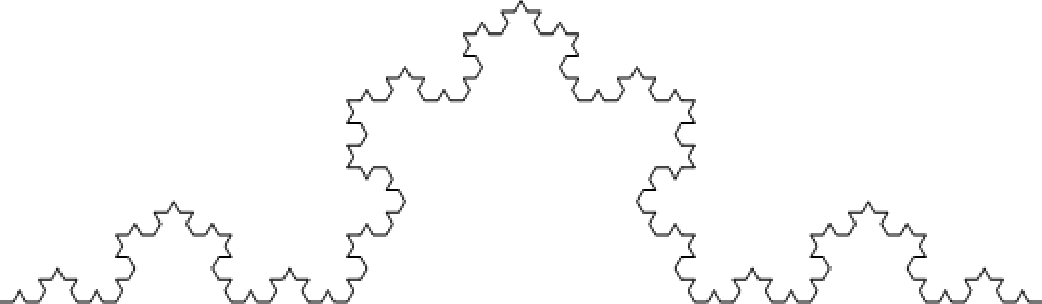
\includegraphics[width=1.0\textwidth]{koch_picture}
\caption{
Chiamato $K_0 \in \RR^2$ il segmento $[0,1]\times \ENCLOSE{0}$,
in figura è rappresentata
la quarta iterata $K_4 = T^4(K_0)$ della contrazione che definisce la curva di K{\"o}ch.
A pagina~\pageref{code:Koch} il codice per generare la figura.
\index{curva di K{\"o}ch}%
}
\label{fig:koch}
\end{figure}

\begin{example}[curva di K{\"o}ch]
Sia $R_\theta\colon \RR^2 \to \RR^2$ la rotazione con centro l'origine di $\theta$ radianti in senso antiorario.
Sia $\alpha = \pi/3$, $p=(1,0)$ e
siano $\phi_1, \phi_2, \phi_3, \phi_4 \colon \RR^2 \to \RR^2$
le funzioni definite da:
\begin{align*}
\phi_1(v) = \frac{v}{3}, \qquad
\phi_2(v) = R_{\alpha}\frac{v}{3} + \phi_1(p), \\
\phi_3(v) = R_{-\alpha}\frac{v}{3} + \phi_2(p), \qquad
\phi_4(v) = \frac{v}{3} + \phi_3(p).
\end{align*}
Allora esiste un unico insieme chiuso $K\subset \RR^2$ tale che
\[
  K = \phi_1(K) \cup \phi_2(K) \cup \phi_3(K) \cup \phi_4(K).
\]
L'insieme $K$ si chiama \emph{curva di K{\"o}ch}%
\mymargin{curva di K{\"o}ch}%
\index{curva di K{\"o}ch}. 
E' un frattale autosimile in quanto è composto da quattro copie riscalate di se stesso.
\end{example}

